\documentclass[11pt,a4paper]{article}
\usepackage[T1]{fontenc}
\usepackage[utf8]{inputenc}
\usepackage[a4paper,margin=2.2cm]{geometry}
\usepackage{lmodern,microtype}
\usepackage{amsmath,amssymb,bm}
\usepackage{booktabs,tabularx,array}
\usepackage{graphicx}
\usepackage{xcolor}
\usepackage[font=small,labelfont=bf]{caption}
\usepackage{enumitem}
\usepackage{hyperref}
\definecolor{accent}{HTML}{00549F}
\hypersetup{colorlinks=true,linkcolor=accent,urlcolor=accent,citecolor=accent,
  pdftitle={Few-shot identification of dynamical systems: technical report},pdfauthor={Elie Rouphael}}
\setlist{itemsep=1pt,topsep=3pt}
\graphicspath{{figures/}}

% Auto-generated by tools/build_report.py from the executed notebook. Do not edit.
\newcommand{\ExplOne}{78.4}
\newcommand{\ExplTwo}{19.4}
\newcommand{\ExplRankTwo}{97.8}
\newcommand{\SigmaHat}{0.0184}
\newcommand{\RtwoPlainOne}{0.96}
\newcommand{\RtwoPlainTwo}{0.35}
\newcommand{\RtwoWhiteOne}{0.98}
\newcommand{\RtwoWhiteTwo}{0.96}
\newcommand{\ScaleVec}{0.0111, 0.0054, 0.0069, 0.3616}
\newcommand{\ScoreMotionCorr}{0.85}
\newcommand{\Threshold}{0.0215}
\newcommand{\InFamilyFlagRate}{5}
\newcommand{\Direction}{-0.16, 0.97, -0.13, -0.15}
\newcommand{\ExNone}{0.0668}
\newcommand{\ExScratch}{0.2799}
\newcommand{\ExContext}{0.0109}
\newcommand{\DetWorst}{5.0\times10^{-3}}
\newcommand{\DetRandom}{2.6\times10^{-4}}
\newcommand{\DetDesigned}{1.1\times10^{-5}}
\newcommand{\CtrlNone}{0.0383 \pm 0.0171}
\newcommand{\CtrlContext}{0.0163 \pm 0.0053}
\newcommand{\CtrlRef}{0.0170 \pm 0.0046}
\newcommand{\ScratchRows}{4 s & 10.4\,\% & 37.3\,\% & 9.8\,\% & 100.0\,\% \\
40 s & 6.4\,\% & 6.2\,\% & 2.7\,\% & 46.9\,\% \\}
\newcommand{\BudgetRows}{1.5 & 0.0554 {\scriptsize[0.037, 0.089]} & 0.1118 {\scriptsize[0.074, 0.179]} & 0.0267 {\scriptsize[0.014, 0.041]} & 0.0027 {\scriptsize[0.001, 0.004]} & 4.2 \\
3 & 0.0534 {\scriptsize[0.034, 0.080]} & 0.0266 {\scriptsize[0.019, 0.064]} & 0.0179 {\scriptsize[0.011, 0.023]} & 0.0024 {\scriptsize[0.001, 0.004]} & 1.5 \\
6 & 0.0581 {\scriptsize[0.036, 0.098]} & 0.0189 {\scriptsize[0.011, 0.062]} & 0.0167 {\scriptsize[0.008, 0.027]} & 0.0023 {\scriptsize[0.001, 0.004]} & 1.1 \\
12 & 0.0461 {\scriptsize[0.026, 0.059]} & 0.0170 {\scriptsize[0.009, 0.027]} & 0.0126 {\scriptsize[0.008, 0.022]} & 0.0022 {\scriptsize[0.001, 0.004]} & 1.3 \\
25 & 0.0522 {\scriptsize[0.029, 0.111]} & 0.0112 {\scriptsize[0.007, 0.018]} & 0.0098 {\scriptsize[0.005, 0.023]} & 0.0026 {\scriptsize[0.001, 0.004]} & 1.1 \\}
\newcommand{\DesignRows}{1.5 & 0.0267 & 0.0279 & 0.0317 & -13.6\,\% & 48\,\% & $[-0.0096,\ +0.0013]$ \\
3 & 0.0301 & 0.0244 & 0.0126 & +48.3\,\% & 73\,\% & $[+0.0076,\ +0.0164]$ \\
6 & 0.0414 & 0.0213 & 0.0126 & +40.8\,\% & 78\,\% & $[+0.0059,\ +0.0118]$ \\
12 & 0.0531 & 0.0160 & 0.0111 & +30.8\,\% & 73\,\% & $[+0.0018,\ +0.0086]$ \\}
\newcommand{\ShiftRows}{0.00 & 0.0164 & 0.0145 & 3\,\% \\
0.10 & 0.0157 & 0.0175 & 23\,\% \\
0.20 & 0.0093 & 0.0198 & 33\,\% \\
0.30 & 0.0078 & 0.0259 & 50\,\% \\
0.40 & 0.0078 & 0.0257 & 73\,\% \\
0.50 & 0.0074 & 0.0295 & 73\,\% \\
0.60 & 0.0069 & 0.0341 & 67\,\% \\}


\newcommand{\R}{\mathbb{R}}
\newcommand{\E}{\mathbb{E}}
\newcommand{\N}{\mathcal{N}}
\newcommand{\etab}{\bar\eta}
\DeclareMathOperator*{\argmin}{arg\,min}
\DeclareMathOperator*{\argmax}{arg\,max}

\title{\textbf{Learning to identify new dynamical systems from a few experiments}\\[4pt]
\large Technical report on the tutorial notebook: pretraining, few-shot adaptation,\\
experiment design, mismatch detection and model-based control}
\author{Elie Rouphael}
\date{}

\begin{document}
\maketitle

\begin{abstract}
\noindent
This report documents the design, mathematics, implementation and results of the notebook
\texttt{few\_shot\_system\_identification\_tutorial.ipynb}. The notebook studies a family of
nonlinear, partially observed, disturbed oscillators and asks whether knowledge extracted from
many previously identified systems can identify a new member of the family from a few seconds of
data. A two-stage pretraining procedure (per-system output-error identification followed by a
principal-component model of the coefficients) yields a two-dimensional task context with an
empirical Gaussian prior. New systems are identified by maximum-a-posteriori estimation of this
context, with a Laplace approximation of its uncertainty. The pretrained model is then used to
design informative experiments via Bayesian D-optimality, to detect systems that the learned family
cannot represent, and to compute feedforward controls. All results are Monte Carlo evaluations over
freshly drawn systems, and every number in this report is produced automatically from the executed
notebook.
\end{abstract}

\tableofcontents
\newpage

%==============================================================================
\section{Motivation and scope}

Foundation models for dynamical systems aim to learn, from data of many heterogeneous systems,
representations that transfer: a new system should be predicted, understood and controlled after
seeing little data of its own. Three sub-problems recur in this programme:
\begin{enumerate}
  \item \textbf{Representation.} What do systems of a kind have in common, and which few quantities
        distinguish one member from another?
  \item \textbf{Adaptation.} How are those quantities inferred for a new system from short, noisy,
        partial observations, and with what uncertainty?
  \item \textbf{Active data collection and reliability.} Which experiment makes the adaptation most
        informative, and how do we notice when the new system lies outside what was learned?
\end{enumerate}
The notebook isolates these questions in a setting small enough that every component can be
written in a few lines, inspected and validated against ground truth. The physics-based model class
used by the learner is deliberately transparent; \S\ref{sec:outlook} discusses how each component
maps to its learned, large-scale counterpart.

\paragraph{Design principles.} (i) The simulator and the learner are strictly separated: the
learner never accesses the true coefficients, the family structure, the velocity or the
disturbance. (ii) The learner's model is \emph{misspecified} (\S\ref{sec:plant}), so that no method
can reach zero error. (iii) Every comparison is made over many freshly drawn systems with paired
designs, and the random baselines are never selected by the criterion they are compared against.

%==============================================================================
\section{The data-generating process}\label{sec:plant}

\subsection{Continuous-time plant}
Each system is a cart on a hardening spring with viscous damping, driven through a saturating
actuator and perturbed by an unknown force. With position $q$ and velocity $v$,
\begin{equation}\label{eq:plant}
  \dot q = v,\qquad
  \dot v = -k q - d v + b\,\varphi(u) - \alpha q^3 \;-\; \gamma q^5 + r + w ,
  \qquad \varphi(u) = 0.3\tanh(u/0.6).
\end{equation}
The coefficients $\eta = [k,\ d,\ b,\ \alpha]^\top$ are those the learner models; the quintic
stiffness $\gamma$, the constant force bias $r$ and the disturbance $w$ are \emph{not} part of the
learner's model. The actuator limits the force to $|\varphi|<0.3$; commands beyond $|u|\approx 1$
produce little additional force, which bounds the admissible excitation.

\subsection{Discretisation}
With sampling time $\Delta t = 0.1$\,s the simulator uses the semi-implicit (symplectic) Euler scheme
with a one-sample input delay,
\begin{equation}\label{eq:disc}
  v_{t+1} = v_t + \Delta t\,a_t(q_t, v_t, u_{t-1}, w_t),\qquad q_{t+1} = q_t + \Delta t\, v_{t+1},
\end{equation}
where $a_t$ is the right-hand side of \eqref{eq:plant}. The natural frequencies in the family are
$\omega_n\approx\sqrt{k}\in[0.8,1.4]$\,rad/s, so $\omega_n\Delta t\le 0.15$, well inside the
stability region ($\omega\Delta t<2$) of the scheme. Every experiment starts at rest from
$q_0=0.2$, $v_0=0$; the initial state is known.

\subsection{Family structure}
The coefficients of a system are generated from a hidden two-dimensional design variable
$c\sim\mathcal U([-1,1]^2)$ and an individual deviation,
\begin{equation}\label{eq:family}
  \eta = \eta_0 + M c + \epsilon,\quad
  \eta_0 = \begin{bmatrix}1.20\\0.32\\0.90\\1.00\end{bmatrix},\quad
  M = \begin{bmatrix}0.55&0.12\\0.07&0.11\\0.16&-0.09\\0.30&0.45\end{bmatrix},\quad
  \epsilon\sim\N\!\big(0,\operatorname{diag}(0.015,0.004,0.008,0.04)^2\big).
\end{equation}
The deviation $\epsilon$ is \emph{off-manifold}: it cannot be represented by any two-dimensional
context. The unmodelled terms are drawn per system as $\gamma\sim\mathcal U[0.035,0.047]$ and
$r = 0.006\,c_1 + 0.002\,\xi$, $\xi\sim\N(0,1)$.

\subsection{Noise and observation}
The disturbance is a coloured AR(1) process and only position is measured:
\begin{equation}
  w_t = \rho\, w_{t-1} + \sigma_w e_t,\qquad y_t = q_t + \nu_t,\qquad
  e_t\sim\N(0,1),\ \nu_t\sim\N(0,\sigma_y^2),
\end{equation}
with $\rho=0.8$, $\sigma_w=0.01$ (stationary standard deviation $\sigma_w/\sqrt{1-\rho^2}\approx0.017$)
and $\sigma_y = 0.01$. Figure~\ref{fig:plant} shows five members of the family and one measured
experiment.

\subsection{Inputs}
All inputs, random or designed, are drawn from the same admissible class: normalised multisines
\begin{equation}\label{eq:multisine}
  u_t = \frac{s_t}{\max_\tau |s_\tau|},\qquad s_t = \sum_{i=1}^{n}\sin(2\pi f_i t\Delta t + \phi_i),\qquad
  \log f_i\sim\mathcal U[\log 0.02,\ \log 0.8],\ \phi_i\sim\mathcal U[0,2\pi],
\end{equation}
with $n=3$ components for experiments on new systems and $n=5$--$6$ for long recordings and
validation. The log-uniform frequency law covers the resonance band ($\approx$0.13--0.22\,Hz)
as well as frequencies far above and below it.

\begin{figure}[t]
  \centering
  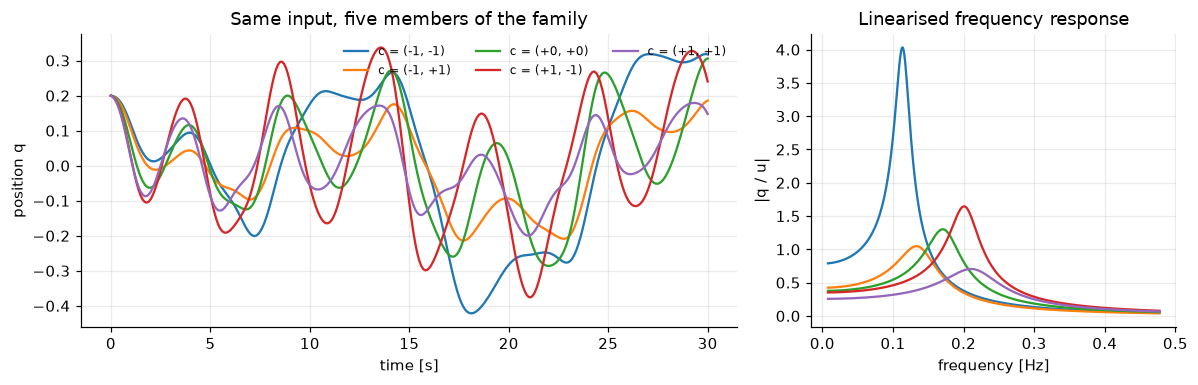
\includegraphics[width=\linewidth]{fig01.png}\\[2pt]
  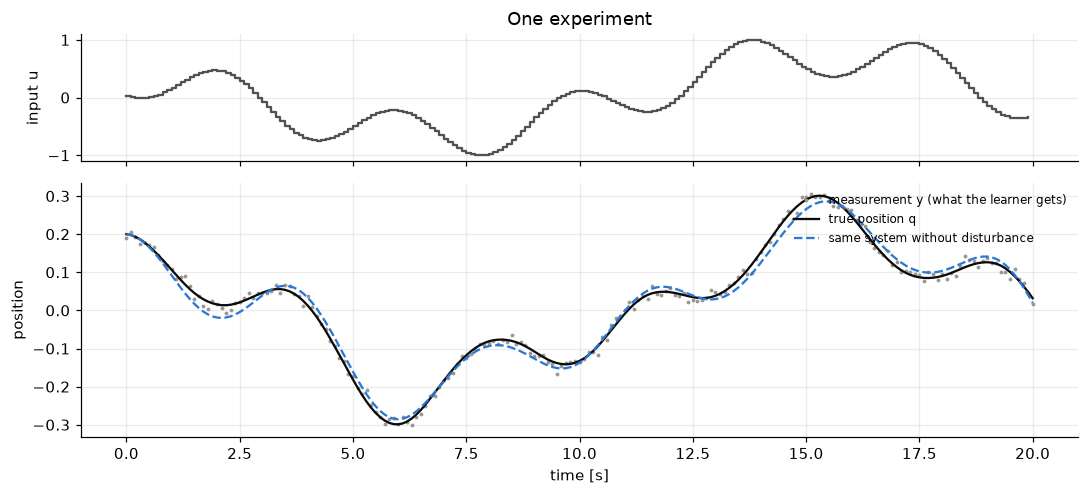
\includegraphics[width=0.9\linewidth]{fig02.png}
  \caption{\textbf{Top:} five members of the family driven by the same input (left) and their
  linearised frequency responses $|0.5\,b/(k-\omega^2+\mathrm{j}d\omega)|$ (right; $0.5=\varphi'(0)$).
  \textbf{Bottom:} one experiment. The learner receives only the grey measurements; the gap between
  the true position and the disturbance-free response is caused by the coloured disturbance.}
  \label{fig:plant}
\end{figure}

%==============================================================================
\section{The learner's model and single-system identification}\label{sec:scratch}

\subsection{Nominal model}
The learner uses \eqref{eq:disc} without $\gamma$, $r$ and $w$, simulated in free run from the known
initial state: $\hat q_t(\eta;u)$ denotes the model's position at time $t$ under input $u$. The
implementation (\texttt{predict}) is vectorised over arbitrary batch dimensions of $\eta$ and $u$,
which later allows all candidate experiments, contexts and finite-difference perturbations to be
simulated in a single time loop.

\subsection{Output-error estimation}
Given one experiment of length $T$,
\begin{equation}\label{eq:oe}
  \hat\eta = \argmin_{\eta\in[\eta_{\min},\eta_{\max}]}\ \sum_{t=0}^{T}\big(y_t-\hat q_t(\eta;u)\big)^2,
\end{equation}
solved with a trust-region reflective method (\texttt{scipy.optimize.least\_squares}) with Jacobian
scaling, box constraints $\eta_{\min}=[0.05,0.01,0.05,0]$, $\eta_{\max}=[5,2,3,5]$ and the generic
initial guess $[1,0.5,1,0.5]$. The Gauss--Newton covariance
$\hat\sigma_i^2(J^\top J)^{-1}$, with $J$ the output Jacobian at the solution and $\hat\sigma_i^2$
the mean squared residual, is returned as a measure of estimation uncertainty. The bounds and the initial guess are deliberately \emph{not} taken
from the family \eqref{eq:family}, so that from-scratch identification uses no information about
it.

\paragraph{Why output error.} An equation-error (regression) formulation would require the velocity
and acceleration, i.e.\ first and second differences of $y$. Their noise variances scale as
$\sigma_y^2/\Delta t^2$ and $\sigma_y^2/\Delta t^4$, and the regressors become noisy
(errors-in-variables bias). Output error avoids differentiation and is the maximum-likelihood
estimator under white measurement noise and a correct model. It is \emph{not} maximum likelihood in the
presence of process noise, for which a prediction-error method with a state estimator (e.g.\ an
extended Kalman filter) would be appropriate. The simpler estimator is kept for transparency, and
its bias is part of what the experiments measure.

\subsection{Identifiability with short data}
Figure~\ref{fig:scratch} repeats \eqref{eq:oe} 30 times on one system with independent inputs and
noise, for 4\,s and 40\,s of data. Table~\ref{tab:scratch} reports the median relative errors.
\begin{table}[h]
  \centering\small
  \caption{Median relative error of from-scratch estimates over 30 repeated experiments on one system.}
  \label{tab:scratch}
  \begin{tabular}{lcccc}
    \toprule
    Data & $k$ & $d$ & $b$ & $\alpha$\\
    \midrule
    \ScratchRows
    \bottomrule
  \end{tabular}
\end{table}

Four seconds are shorter than one oscillation period ($2\pi/\omega_n\approx4.5$--$8$\,s): the
output sensitivities $\partial\hat q/\partial\eta_j$ are nearly collinear, the Gauss--Newton matrix
is ill-conditioned, and many coefficient vectors explain the data equally well. The cubic
coefficient $\alpha$ is weakly identifiable even with 40\,s of data: with 4\,s its estimates collapse
onto the bounds, and with 40\,s they are still off by tens of percent. Its regressor $q^3$ matters
only at the largest deflections, and it is confounded with the unmodelled quintic term
$\gamma q^5$ and with the disturbance.

\begin{figure}[t]
  \centering
  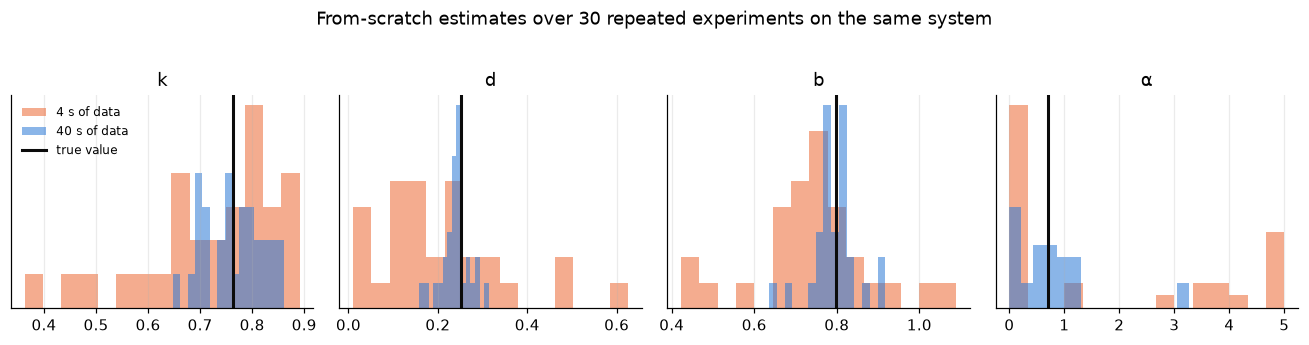
\includegraphics[width=\linewidth]{fig03.png}
  \caption{From-scratch estimates over 30 repeated experiments on the same system (vertical line:
  true value). Short experiments leave the coefficients poorly determined; $\alpha$ remains
  uncertain with long data.}
  \label{fig:scratch}
\end{figure}

%==============================================================================
\section{Pretraining: a low-dimensional model of the family}\label{sec:pretrain}

\subsection{Two-stage procedure}
Twenty training systems are drawn from the family and each is recorded for 80\,s under a
six-component multisine. Pretraining proceeds in two stages.
\begin{enumerate}
  \item \textbf{Per-system identification:} $\hat\eta_i$ and its Gauss--Newton covariance $P_i$
  from \eqref{eq:oe}, $i=1,\dots,N$, $N=20$.
  \item \textbf{Noise-whitened principal component model.} Let $s_j=\big(\frac1N\sum_i (P_i)_{jj}\big)^{1/2}$
  be the average estimation standard deviation of coefficient $j$ and $D=\operatorname{diag}(s)$.
  With $\etab=\frac1N\sum_i\hat\eta_i$ and the SVD of the scaled, centred matrix
  $X=[D^{-1}(\hat\eta_1-\etab),\dots,D^{-1}(\hat\eta_N-\etab)]^\top = W\Sigma V^\top$, the sample
  covariance of $X$ has eigenvalues $\lambda_j=\Sigma_{jj}^2/(N-1)$. For rank $r=2$,
  \begin{equation}\label{eq:pca}
    U = D\,V_{:,1:r}\,\Lambda_r^{1/2},\qquad z_i = \Lambda_r^{-1/2}V_{:,1:r}^\top D^{-1}(\hat\eta_i-\etab),\qquad
    \hat\eta_i\approx\etab + U z_i .
  \end{equation}
\end{enumerate}

\paragraph{Why noise whitening.} The spread of the estimates $\hat\eta_i$ has two sources:
genuine differences between systems and estimation error. Plain PCA ($D=I$) ranks directions by raw
spread and therefore allocates a principal direction to the scatter of the poorly identified
$\alpha$, whose estimation standard deviation is one to two orders of magnitude larger than those of
$k$, $d$ and $b$ (here $s=[\ScaleVec]$). Scaling by $s$ ranks directions by
signal-to-noise ratio instead. This is the homoscedastic special case of factor analysis with known
noise variances, and a first-order substitute for the joint hierarchical model discussed below.

The whitening by $\Lambda_r^{-1/2}$ makes the training contexts have identity sample covariance, so
$z\sim\N(0,I)$ is the Gaussian population model implied by the training set: an empirical-Bayes
prior for new systems. Finally, the pooled residual level
$\hat\sigma^2 = \frac1N\sum_i \frac{1}{T+1}\sum_t (y_{i,t}-\hat q_t(\hat\eta_i))^2$ estimates the
effective noise the adapted model should expect. It includes measurement noise, the effect of the
disturbance on the free-run output, and model mismatch, and is therefore larger than $\sigma_y$.

\subsection{Results}
The first two principal directions explain \ExplOne\,\% and \ExplTwo\,\% of the noise-weighted
variance (\ExplRankTwo\,\% together), and $\hat\sigma=\SigmaHat$ (versus $\sigma_y=0.01$).
Figure~\ref{fig:pretrain} shows that $k$, $d$ and $b$ are recovered well from long recordings while
$\alpha$ is only roughly determined, and that the learned contexts vary smoothly with the hidden
design variables. They are a rotated and rescaled version of $c$, which is all that can be expected:
the likelihood is invariant to invertible reparameterisations of the context.

Table~\ref{tab:pca} quantifies how much of each hidden design variable is explained by an affine
function of the learned contexts. Noise whitening is decisive for the second design variable, which
acts mainly through the poorly identified $\alpha$ and the small damping variations.

\begin{table}[h]
  \centering\small
  \caption{Coefficient of determination $R^2$ of the hidden design variables regressed (affinely) on
  the learned training contexts.}
  \label{tab:pca}
  \begin{tabular}{lcc}
    \toprule
    Family model & $c_1$ & $c_2$\\
    \midrule
    plain PCA & \RtwoPlainOne & \RtwoPlainTwo\\
    noise-whitened PCA & \RtwoWhiteOne & \RtwoWhiteTwo\\
    \bottomrule
  \end{tabular}
\end{table}

\paragraph{Relation to hierarchical models.} The two-stage estimator approximates a linear mixed-effects
(hierarchical Bayesian) model $\eta_i = \etab + Uz_i + \epsilon_i$, $z_i\sim\N(0,I)$, fitted by
treating the stage-one estimates as data. A joint estimator (e.g.\ expectation--maximisation over all
trajectories) would propagate the full per-system estimation covariances $P_i$, including their
correlations and their variation across systems. Noise-whitened PCA uses only the average marginal
variances, which suffices here to stop poorly identified coefficients from inflating the apparent
family variance.

\begin{figure}[t]
  \centering
  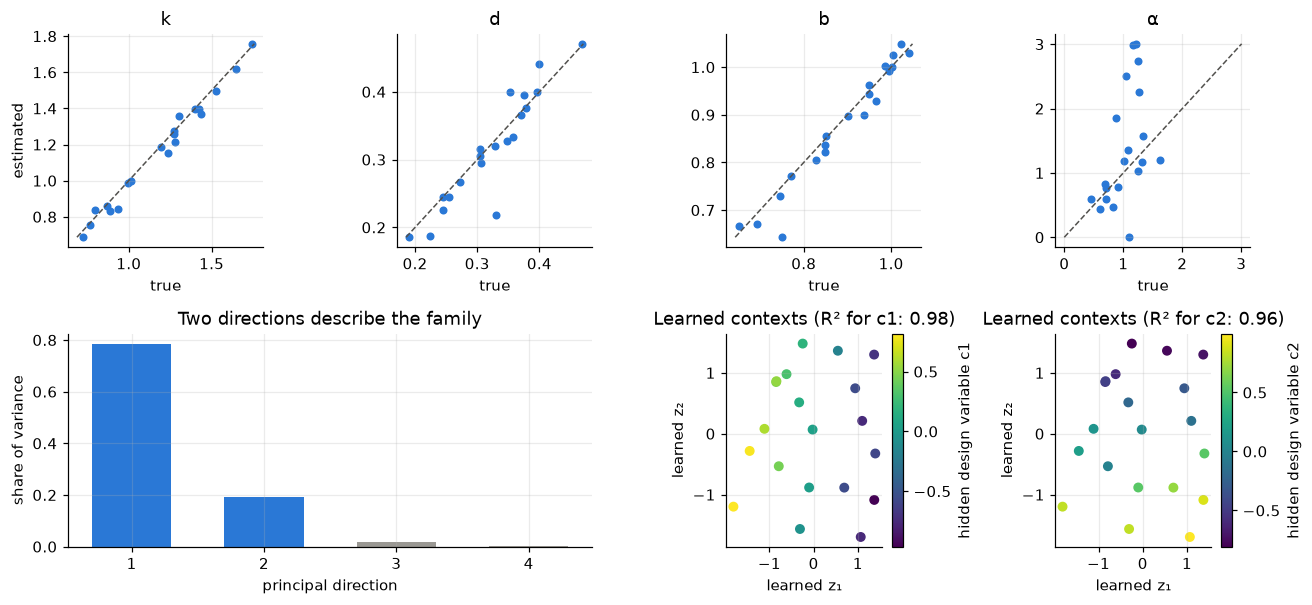
\includegraphics[width=\linewidth]{fig04.png}
  \caption{Pretraining. \textbf{Top:} per-system estimates versus truth. \textbf{Bottom left:}
  explained variance per principal direction. \textbf{Bottom right:} learned contexts coloured by
  the hidden design variables $c_1$, $c_2$.}
  \label{fig:pretrain}
\end{figure}

%==============================================================================
\section{Few-shot adaptation}\label{sec:adapt}

\subsection{MAP estimation of the context}
For a new system, $\etab$, $U$ and $\hat\sigma$ are frozen and only $z$ is estimated:
\begin{equation}\label{eq:map}
  \hat z = \argmin_{z\in\R^2}\ \frac{1}{\hat\sigma^2}\sum_{t=0}^{T}\big(y_t-\hat q_t(\mathcal D(z);u)\big)^2+\|z\|^2,
  \qquad \mathcal D(z)=\operatorname{clip}\big(\etab+Uz,\ \eta_{\min},\eta_{\max}\big).
\end{equation}
The problem is solved as a stacked least-squares problem with residual
$[\,(y-\hat q(\mathcal D(z)))/\hat\sigma;\ z\,]$ from $z=0$ (the population mean). The clipping keeps
decoded coefficients physical, e.g.\ $\alpha\ge0$; a negative hardening coefficient would make the
model diverge for large deflections.

\subsection{Laplace approximation}
With $S=\partial\hat q/\partial z\in\R^{(T+1)\times2}$ evaluated at $\hat z$ (finite differences
inside the solver), the Gauss--Newton approximation of the negative log-posterior Hessian gives
\begin{equation}\label{eq:laplace}
  \operatorname{Cov}(z\mid y)\approx\Big(\hat\sigma^{-2}S^\top S + I\Big)^{-1}.
\end{equation}
This expression assumes independent residuals. With coloured disturbances the effective number of
independent samples is smaller than $T+1$, so \eqref{eq:laplace} is expected to be overconfident
(\S\ref{sec:limits}).

\subsection{Why it helps}
Two effects combine. The number of unknowns drops from four to two, which lowers variance. The prior
restricts estimates to the region occupied by the family, which regularises directions the data
cannot resolve. The price is bias whenever the new system is not representable as
$\etab+Uz$: the off-manifold deviation $\epsilon$, the stage-one estimation errors, and in
\S\ref{sec:detect} deliberate shifts.

In the single example of Figure~\ref{fig:adapt} (2\,s of data, a third of an oscillation period),
the validation RMSE is \ExNone\ with no adaptation, \ExScratch\ from scratch and \ExContext\ with the
adapted context. The from-scratch fit explains the short record with the coefficients of a much
less damped oscillator, and its free-run prediction drifts away. The adapted context stays within
the family and extrapolates well.

\begin{figure}[t]
  \centering
  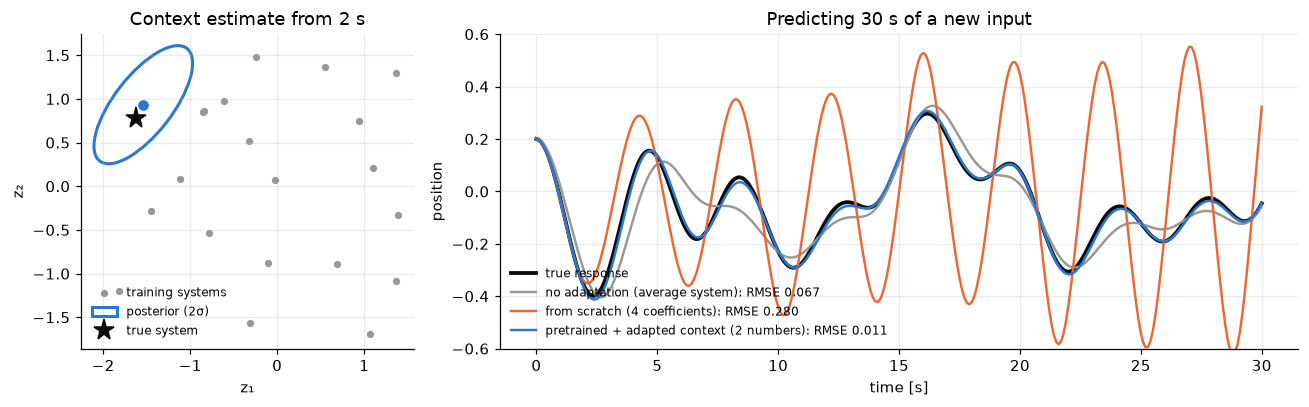
\includegraphics[width=\linewidth]{fig05.png}
  \caption{Adaptation from 2\,s of data. \textbf{Left:} MAP context, 2$\sigma$ Laplace ellipse, and
  the projection of the true coefficients onto the learned plane (star). \textbf{Right:} prediction
  of the disturbance-free response to a new 30\,s input.}
  \label{fig:adapt}
\end{figure}

%==============================================================================
\section{Evaluation protocol}\label{sec:protocol}

\begin{itemize}
  \item \textbf{Fresh systems.} Every trial draws a new system from \eqref{eq:family}; no test system
        is used for pretraining.
  \item \textbf{Metric.} Models are compared on a fresh 30\,s, six-component multisine by the RMSE
        between the model prediction $\hat q_t(\hat\eta)$ and the system's \emph{disturbance-free}
        response ($w\equiv0$, $\nu\equiv0$, but $\gamma$ and $r$ present). This isolates model quality
        from the unpredictable disturbance realisation.
  \item \textbf{Reference.} The true $\eta$ inserted in the nominal model gives the error due to
        $\gamma$ and $r$ alone. It is a reference, not a lower bound: a fitted model can partly
        compensate unmodelled terms.
  \item \textbf{Pairing.} Within a trial all methods are evaluated on the same system and the same
        validation input. In the data-budget study they also share the same experiment; in the
        design study each method runs its own experiment with independent noise.
  \item \textbf{Fair baselines.} Random experiments are drawn from the same admissible class and are
        never scored. Designed experiments are selected before the new system is excited.
  \item \textbf{Uncertainty.} Medians with inter-quartile ranges, paired win rates, and percentile
        bootstrap intervals (5000 resamples) of mean paired differences.
\end{itemize}

%==============================================================================
\section{Data-budget study}\label{sec:budget}

For $T\in\{15,30,60,120,250\}$ samples (1.5--25\,s) and 40 systems per budget, one random
three-component experiment is run per system and four predictors are compared: no adaptation
($\etab$), from scratch \eqref{eq:oe}, pretrained context \eqref{eq:map}, and the reference.

\begin{table}[h]
  \centering\small
  \caption{Validation RMSE, median [IQR] over 40 new systems per budget. Last column: ratio of the
  from-scratch to the pretrained median.}
  \label{tab:budget}
  \begin{tabular}{r@{\ \ }cccc@{\ \ }c}
    \toprule
    $T\Delta t$ [s] & no adaptation & from scratch & pretrained + context & reference & ratio\\
    \midrule
    \BudgetRows
    \bottomrule
  \end{tabular}
\end{table}

\begin{figure}[t]
  \centering
  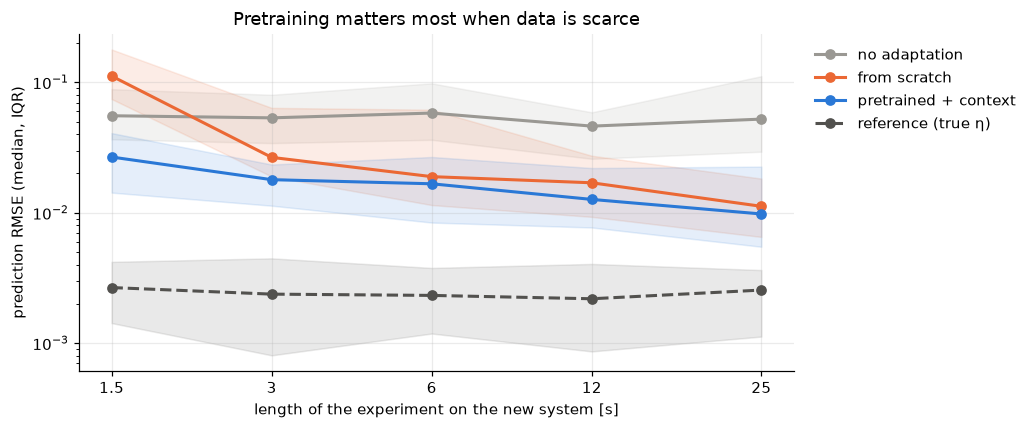
\includegraphics[width=0.72\linewidth]{fig06.png}
  \caption{Validation error against the length of the experiment on the new system (log--log;
  lines: medians, bands: inter-quartile ranges).}
  \label{fig:budget}
\end{figure}

Table~\ref{tab:budget} and Figure~\ref{fig:budget} show the characteristic few-shot pattern. With
scarce data, from-scratch identification overfits and is worse than using the population mean,
while the pretrained context already halves the error of the population mean. As the budget grows,
the from-scratch estimator improves faster and the ratio in the last column falls from about four
towards one: pretraining buys \emph{data efficiency}, and in this setting it remains at least as good
as identification from scratch at every budget tested. Both learned predictors remain above the
reference. The residual gap is structural (stage-one errors in $\etab,U$, the rank restriction, and
the poorly determined $\alpha$) and cannot be removed by more data on the new system.

%==============================================================================
\section{Experiment design}\label{sec:design}

\subsection{Criterion}
For additive Gaussian output noise, the Fisher information of the context under input $u$, including
the unit prior precision, is
\begin{equation}\label{eq:fisher}
  \mathcal I(u;z) = \hat\sigma^{-2}S(u;z)^\top S(u;z) + I,\qquad S_{tj}(u;z)=\frac{\partial\hat q_t(\mathcal D(z);u)}{\partial z_j},
\end{equation}
the inverse of the Laplace covariance \eqref{eq:laplace} evaluated before the data are seen. Since
$z$ is unknown, the design maximises the prior expectation of the log-determinant (Bayesian
D-optimality), approximating the prior by the $N=20$ training contexts:
\begin{equation}\label{eq:dopt}
  u^\star=\argmax_{u\in\mathcal C}\ J(u),\qquad J(u)=\frac1N\sum_{i=1}^{N}\log\det\mathcal I(u;z_i).
\end{equation}
For a model linearised around $z$, $\tfrac12\log\det\mathcal I(u;z)$ equals the expected information
gain (mutual information between $z$ and $y$) under the prior $\N(0,I)$, so $J$ is a local-linear
approximation of the expected information gain of the experiment.

\subsection{Implementation}
The sensitivities are computed by central differences ($\varepsilon=10^{-4}$) in both context
directions. One vectorised call of the model simulates all $|\mathcal C|\times N\times 2\times2$
trajectories in a single loop over time, so scoring 200--300 candidates takes a fraction of a
second. The optimiser is random search: $u^\star$ is the best of a pool $\mathcal C$ of admissible
multisines \eqref{eq:multisine}. For illustration, the worst candidate ($\argmin J$) is also
retained.

\subsection{Physical interpretation}
Figure~\ref{fig:design} shows the score distribution of 300 four-second candidates. The score
correlates with how much the candidate moves the average system (correlation \ScoreMotionCorr),
since a system that does not move produces outputs that are insensitive to its coefficients. The
best candidates swing the cart through large, two-sided deflections at low frequency and near
resonance. The worst shake it at high frequency, which the mass filters out. The correlation is not
perfect: the \emph{shape} of the motion determines which directions of $z$ become distinguishable.
In the example of Figure~\ref{fig:ellipses}, the determinant of the posterior covariance is
$\DetWorst$ (worst), $\DetRandom$ (random) and $\DetDesigned$ (designed).

The same figure exposes a limitation: the smallest (designed) ellipse does not contain the
projection of the true coefficients. The Laplace posterior is overconfident, because
\eqref{eq:laplace} treats the residuals as white and the model as correct, while the disturbance is
coloured and $\gamma$, $r$ are missing. A smaller ellipse therefore signals more information, but its
absolute size cannot be trusted as a calibrated uncertainty (\S\ref{sec:limits}).

\begin{figure}[t]
  \centering
  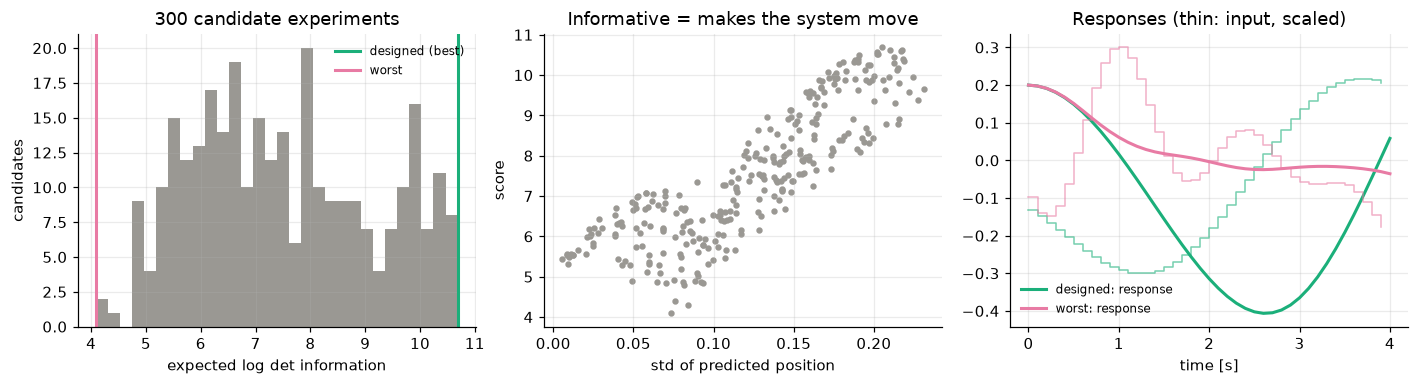
\includegraphics[width=\linewidth]{fig07.png}
  \caption{\textbf{Left:} scores of 300 candidate experiments. \textbf{Centre:} score versus the
  standard deviation of the predicted motion of the average system. \textbf{Right:} responses of the
  average system to the best and worst candidate (thin lines: scaled inputs).}
  \label{fig:design}
\end{figure}

\begin{figure}[t]
  \centering
  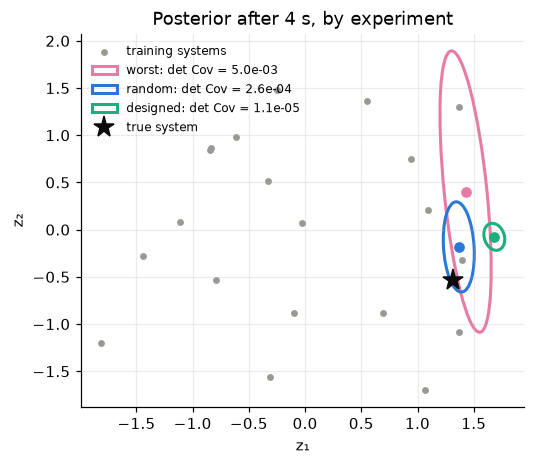
\includegraphics[width=0.5\linewidth]{fig08.png}
  \caption{Posterior (2$\sigma$ Laplace ellipses) for one new system after 4\,s under the worst, a
  random and the designed experiment (star: projection of the true coefficients).}
  \label{fig:ellipses}
\end{figure}

\subsection{Monte Carlo evaluation}
For $T\in\{15,30,60,120\}$ and 60 new systems per budget, each trial draws a fresh pool of 200
candidates, selects the designed and the worst experiment, draws an unscored random experiment, and
adapts the context from each. Table~\ref{tab:design} reports the mean validation RMSE, the relative
reduction of the designed over the random experiment, the paired win rate, and a bootstrap
interval for the mean paired reduction.

\begin{table}[h]
  \centering\small
  \caption{Pretrained context adaptation under different experiments (60 new systems per budget).}
  \label{tab:design}
  \begin{tabular}{rccccc c}
    \toprule
    $T\Delta t$ [s] & worst & random & designed & reduction & designed wins & 95\,\% CI (random $-$ designed)\\
    \midrule
    \DesignRows
    \bottomrule
  \end{tabular}
\end{table}

\begin{figure}[t]
  \centering
  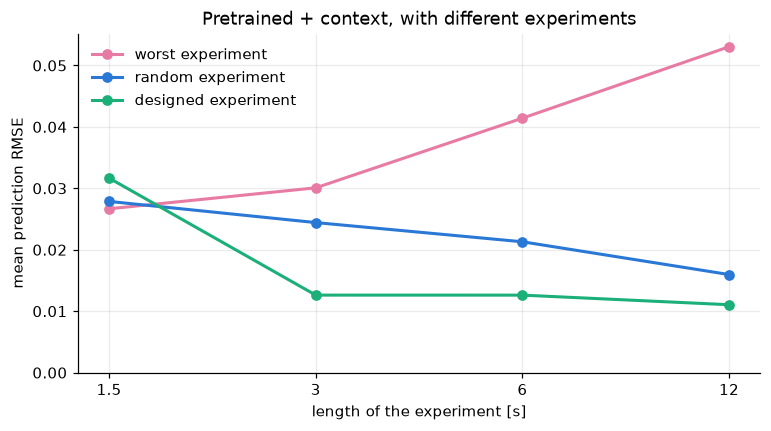
\includegraphics[width=0.72\linewidth]{fig09.png}
  \caption{Mean validation RMSE of the adapted model for the worst, random and designed experiment.}
  \label{fig:designmc}
\end{figure}

The value of design depends on the budget. With 1.5\,s (a quarter of an oscillation period) no
experiment reveals much, the prior dominates, and the difference between designed and random
experiments is not significant: the bootstrap interval contains zero. From 3\,s on, the designed
experiment lowers the mean error by roughly a third to a half, wins about three quarters of the
paired trials, and all bootstrap intervals exclude zero, while the worst experiments waste most of
the data. The relative advantage is largest for the shortest informative experiments and decreases
as the experiment grows, since random inputs then also accumulate enough information. The designed
experiment does not win every paired trial. The criterion targets parameter uncertainty under a
linearised, white-noise model rather than the validation error itself, and mismatch and coloured
disturbances remain.

%==============================================================================
\section{Detecting systems outside the learned family}\label{sec:detect}

\subsection{Construction of out-of-family systems}
Let $V_\perp\in\R^{4\times2}$ be an orthonormal basis of the orthogonal complement of
$\operatorname{span}(U)$ (from a full SVD of $U$). The column with the largest damping component,
signed to increase damping, defines a direction $n$ that no context can express. The direction
realised in the run is $n=[\Direction]^\top$ in $[k,d,b,\alpha]$. Test systems are drawn from the
family and shifted, $\eta\leftarrow\operatorname{clip}(\eta+\delta n)$, for seven values
$\delta\in\{0,0.1,\dots,0.6\}$, 30 systems each, with 12\,s random experiments. The shift is measured in raw
coefficient units, which weights coefficients by their natural scale; a normalised metric would be a
natural refinement.

\subsection{Misfit test}
After adaptation, the RMS output misfit $m=\big(\frac1{T+1}\sum_t(y_t-\hat q_t(\mathcal D(\hat z)))^2\big)^{1/2}$
is compared with the threshold $\tau=\Threshold$, the empirical 95\,\% quantile of $m$ over 60
in-family systems under the same protocol (nominal false-alarm rate 5\,\%; realised rate on the
calibration set: \InFamilyFlagRate\,\%). A system is flagged if $m>\tau$.

\begin{table}[h]
  \centering\small
  \caption{Out-of-family shifts: median validation RMSE and share of systems flagged by the misfit test.}
  \label{tab:shift}
  \begin{tabular}{cccc}
    \toprule
    $\delta$ & from scratch & pretrained + context & flagged\\
    \midrule
    \ShiftRows
    \bottomrule
  \end{tabular}
\end{table}

\begin{figure}[t]
  \centering
  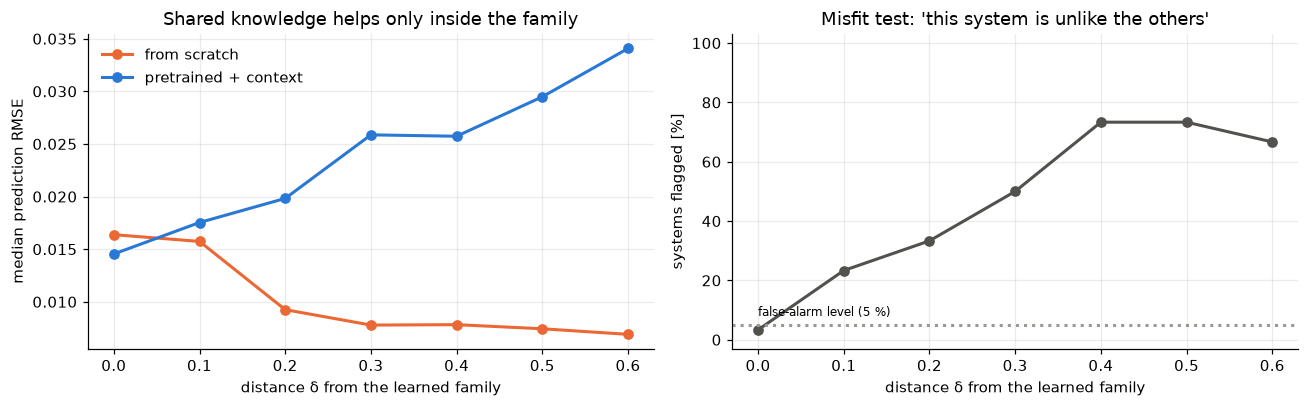
\includegraphics[width=\linewidth]{fig10.png}
  \caption{\textbf{Left:} prediction error as the new system moves away from the learned family.
  \textbf{Right:} share of systems flagged by the misfit test (dotted: nominal false-alarm level).}
  \label{fig:shift}
\end{figure}

Table~\ref{tab:shift} and Figure~\ref{fig:shift} show the trade-off. The pretrained model is only
as good as its family: as $\delta$ grows, its error grows because the prior and the
two-dimensional parameterisation force a biased estimate. The from-scratch estimator makes no
family assumption and is insensitive to $\delta$. Its error even decreases, as more strongly damped
systems move less. With 12\,s of data from scratch is already competitive inside the family, so the
pretrained model loses its advantage after a small shift. The misfit statistic grows with $\delta$
because the best representable model can no longer explain the data. The flag rate rises from the
nominal false-alarm level at $\delta=0$ to roughly three quarters of the systems for large shifts.
Detection, however, lags degradation: at moderate shifts the adapter is already worse than from
scratch while most systems still pass the test, because the disturbance-induced misfit varies
strongly from system to system. The resulting switching rule between the small adapter and full
identification is sound in principle, but its power is limited; innovation-based tests that
whiten the coloured residuals would be a natural improvement.

%==============================================================================
\section{Model-based feedforward control}\label{sec:control}

To test whether model quality carries over to control, each candidate model computes a
feedforward input that tracks a smooth reference $r_t$ (logistic transitions
$0.2\to-0.15\to0.1$ over 12\,s):
\begin{equation}\label{eq:ff}
  u^\star(\hat\eta)=\argmin_{u\in[-2,2]^{T}}\ \sum_{t=0}^{T}\big(\hat q_t(\hat\eta;u)-r_t\big)^2+\lambda\sum_{t=0}^{T-2}(u_{t+1}-u_t)^2,
  \qquad\lambda=0.05 .
\end{equation}
The $T=120$ decision variables are optimised by trust-region least squares with a Jacobian obtained
by forward differences, computed in one vectorised batch of $T+1$ model rollouts. The input is then
applied open loop to the \emph{true} system, including disturbances. Open-loop feedforward cannot
correct model errors during execution, which makes the tracking error a direct measure of model
quality. The adapted model uses one designed 6\,s experiment per system.

Over 15 new systems the tracking RMSE (mean $\pm$ standard deviation) is $\CtrlNone$ with the
average-system model, $\CtrlContext$ with the adapted model, and $\CtrlRef$ with the true
coefficients (Figure~\ref{fig:control}). Six seconds of designed data more than halve the tracking
error of the average-system model and match the true coefficients. The adapted model can be
marginally better, since it is fitted to the actual behaviour and partly compensates the
unmodelled terms. The remaining error stems from the disturbance and the unmodelled terms, which
only feedback can reject.

\begin{figure}[t]
  \centering
  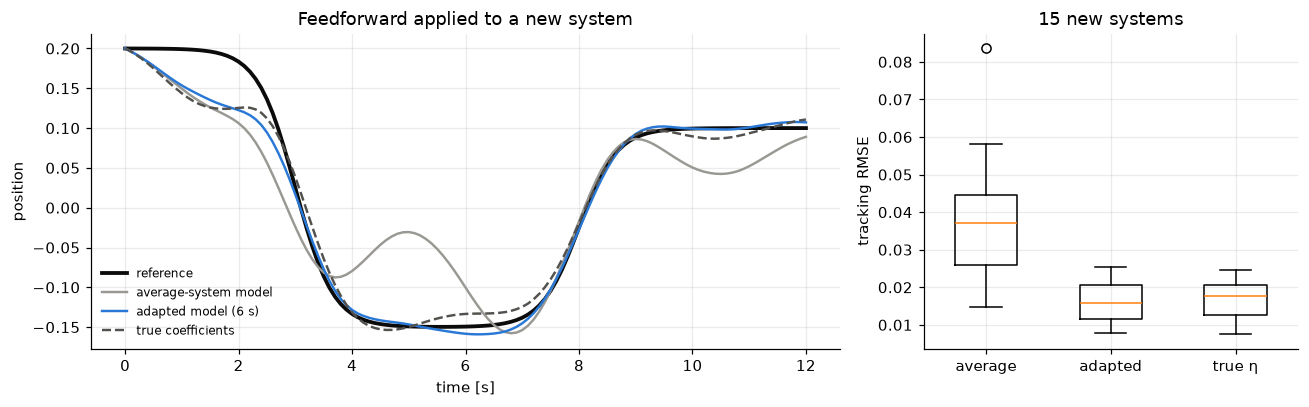
\includegraphics[width=\linewidth]{fig11.png}
  \caption{\textbf{Left:} feedforward tracking on one new system with three models.
  \textbf{Right:} tracking RMSE over 15 new systems.}
  \label{fig:control}
\end{figure}

%==============================================================================
\section{Limitations}\label{sec:limits}

\begin{itemize}
  \item \textbf{Known model class.} The learner knows the structure of the dominant physics. A
        learned backbone (neural state-space or sequence model) removes this assumption but makes
        identifiability and extrapolation harder to analyse.
  \item \textbf{Two-stage pretraining.} Stage-one errors (notably in $\alpha$) enter $\etab$ and $U$
        as if they were genuine family variation. Noise-whitened PCA mitigates this with average
        marginal variances only; a joint hierarchical estimator would use the full per-system
        covariances.
  \item \textbf{Output error under process noise.} The estimator is not maximum likelihood when
        disturbances act on the state. Prediction-error methods with state estimation are the
        principled alternative.
  \item \textbf{Calibration.} The Laplace covariance assumes white residuals, while the disturbance
        is coloured and the model misspecified; Figure~\ref{fig:ellipses} shows an ellipse that misses
        the true system. Coverage should be measured, not assumed.
  \item \textbf{Design.} The criterion is local (linearised), parameter-oriented (D-optimal) and
        optimised by random search over one input class. It does not account for safety constraints
        on state or input beyond the actuator limit.
  \item \textbf{Linear family model.} PCA represents the family as an affine plane; curved families
        require nonlinear decoders (e.g.\ variational autoencoders or hypernetworks).
  \item \textbf{Scale.} One family, one seed and moderate Monte Carlo sizes; conclusions are
        illustrative, not general.
\end{itemize}

%==============================================================================
\section{From the tutorial to foundation models}\label{sec:outlook}

\begin{table}[h]
  \centering\small
  \begin{tabularx}{\linewidth}{l X X}
    \toprule
    Component & In the notebook & Scalable counterpart\\
    \midrule
    Model class & known physics, 4 coefficients & structured neural state-space / sequence models\\
    Pretraining & per-system identification + noise-whitened PCA & joint training across heterogeneous systems and sensors\\
    Task context & $z\in\R^2$, prior $\N(0,I)$ & learned context encoders, low-rank adapters, hypernetworks\\
    Adaptation & MAP + Laplace & amortised inference, fast gradient adaptation, in-context learning\\
    Experiment design & Bayesian D-optimal random search & safe, constrained, sequential Bayesian design\\
    Reliability & misfit test with calibrated threshold & calibrated uncertainty, out-of-distribution detection\\
    Use & open-loop feedforward & MPC, reinforcement learning, safe learning-based control\\
    \bottomrule
  \end{tabularx}
\end{table}

\paragraph{Research questions raised by the experiments.}
\begin{enumerate}
  \item \emph{Identifiability of learned contexts:} under which conditions on the backbone and the
        excitation can the context of a new system be recovered from partial, noisy observations, and
        with what sample complexity?
  \item \emph{Calibrated uncertainty under coloured noise and mismatch:} how can posteriors over
        contexts be made trustworthy enough for decisions (design, control, safety)?
  \item \emph{Safe and goal-oriented excitation:} how should information gain be traded against
        state/input constraints and against the downstream task (prediction, control)?
  \item \emph{Adaptive capacity:} how can a model decide online that its adapter is insufficient,
        and grow it with guarantees on false alarms?
  \item \emph{Closing the loop:} how should identification, uncertainty and control be designed
        jointly, e.g.\ dual control, with stability guarantees for the adapted model?
\end{enumerate}

%==============================================================================
\appendix
\section{Reproducibility}

\begin{itemize}\sloppy
  \item \textbf{Build.} \texttt{python tools/build\_report.py} regenerates the notebook from
        \texttt{tools/build\_tutorial\_notebook.py}, executes it, exports the figures and
        \texttt{report/tutorial\_metrics.json}, writes \texttt{report/results.tex} and compiles this
        document. All numbers in the text and tables are macros from that file.
  \item \textbf{Randomness.} A single generator seeded with 2026 drives all draws, in notebook
        order.
  \item \textbf{Dependencies.} NumPy, SciPy, Matplotlib; for building: nbformat, nbclient,
        ipykernel, pdflatex.
  \item \textbf{Runtime.} About two minutes on a laptop CPU, dominated by the Monte Carlo studies.
\end{itemize}

\begin{table}[h]
  \centering\small
  \caption{Default configuration.}
  \begin{tabular}{ll}
    \toprule
    Sampling time & $\Delta t=0.1$\,s, initial state $(0.2, 0)$\\
    Noise & $\sigma_y=0.01$, $\sigma_w=0.01$, $\rho=0.8$\\
    Pretraining & 20 systems $\times$ 40\,s, six-component multisines, rank 2\\
    Data-budget study & $T\in\{15,30,60,120,250\}$, 40 systems each\\
    Design study & $T\in\{15,30,60,120\}$, 60 systems each, 200 candidates per trial\\
    Out-of-family study & 7 shifts $\delta\in[0,0.6]$, 30 systems each, $T=120$; 60 calibration systems\\
    Control study & 15 systems, $T=120$, $\lambda=0.05$, 6\,s designed identification experiment\\
    Validation & fresh 30\,s six-component multisine, disturbance-free response\\
    \bottomrule
  \end{tabular}
\end{table}

\end{document}
